\section{}
\[
H(s)=\frac{100\,(s+1)}{s^2+20s+100}=\frac{100\,(s+1)}{(s+10)^2}\,.
\]
\subsection{Bode-Diagramm}
\begin{center}
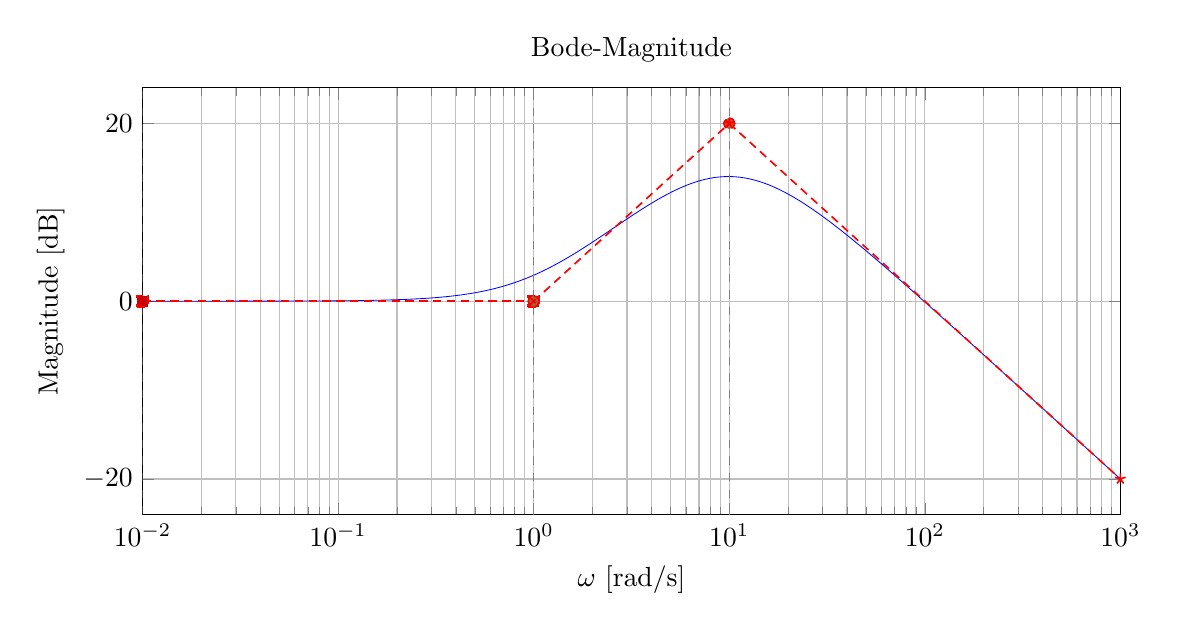
\begin{tikzpicture}
\begin{semilogxaxis}[
  width=14cm,height=7cm,
  xmin=1e-2,xmax=1e3,
  xlabel={$\omega$ [rad/s]},
  ylabel={Magnitude [dB]},
  grid=both,
  ytick distance=20,
  title={Bode-Magnitude}
]
\addplot[
  domain=1e-2:1e3,
  samples=600,
  mark=none,
  line width=0.3pt,
  blue
] {40 + 20*ln(sqrt(1 + x^2))/ln(10) - 40*ln(sqrt(100 + x^2))/ln(10)};
\addplot+[domain=1e-2:1,samples=2,dashed,dash pattern=on 3pt off 2pt,line width=0.6pt,red] {0};
\addplot+[domain=1:1e1,samples=2,dashed,dash pattern=on 3pt off 2pt,line width=0.6pt,red] {20*ln(x)/ln(10)};
\addplot+[domain=1e1:1e3,samples=2,dashed,dash pattern=on 3pt off 2pt,line width=0.6pt,red] {20 - 20*ln(x/10)/ln(10)};
\draw[gray,dashed] (rel axis cs:0,0) -- (rel axis cs:0,1);
\draw[gray,dashed] (axis cs:1,\pgfkeysvalueof{/pgfplots/ymin}) -- (axis cs:1,\pgfkeysvalueof{/pgfplots/ymax});
\draw[gray,dashed] (axis cs:10,\pgfkeysvalueof{/pgfplots/ymin}) -- (axis cs:10,\pgfkeysvalueof{/pgfplots/ymax});
\node[gray,anchor=south east] at (axis cs:1,\pgfkeysvalueof{/pgfplots/ymax}) {\scriptsize Nullstelle $\omega_z=1$};
\node[gray,anchor=south east] at (axis cs:10,\pgfkeysvalueof{/pgfplots/ymax}) {\scriptsize Pol $\omega_p=10$ (doppelt)};
\end{semilogxaxis}
\end{tikzpicture}
\vspace{6mm}
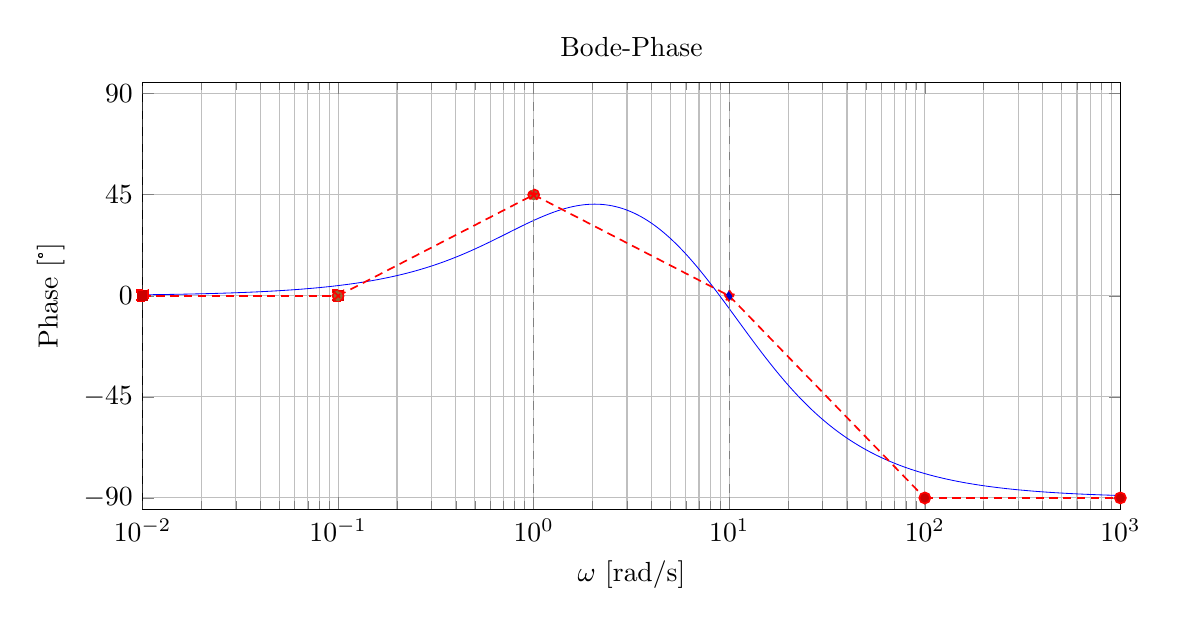
\begin{tikzpicture}
\begin{semilogxaxis}[
  width=14cm,height=7cm,
  xmin=1e-2,xmax=1e3,
  ymin=-95,ymax=95,
  ytick distance=45,
  xlabel={$\omega$ [rad/s]},
  ylabel={Phase [°]},
  grid=both,
  title={Bode-Phase}
]
\addplot[
  domain=1e-2:1e3,
  samples=600,
  mark=none,
  line width=0.3pt,
  blue
] {atan(x) - 2*atan(x/10)};
\addplot+[domain=1e-2:1e-1,samples=2,dashed,dash pattern=on 3pt off 2pt,line width=0.6pt,red] {0};
\addplot+[domain=1e-1:1e0,samples=2,dashed,dash pattern=on 3pt off 2pt,line width=0.6pt,red] {45 + 45*ln(x)/ln(10)};
\addplot+[domain=1e0:1e1,samples=2,dashed,dash pattern=on 3pt off 2pt,line width=0.6pt,red] {45 - 45*ln(x)/ln(10)};
\addplot+[domain=1e1:1e2,samples=2,dashed,dash pattern=on 3pt off 2pt,line width=0.6pt,red] {-90*ln(x/10)/ln(10)};
\addplot+[domain=1e2:1e3,samples=2,dashed,dash pattern=on 3pt off 2pt,line width=0.6pt,red] {-90};
\draw[gray,dashed] (rel axis cs:0,0) -- (rel axis cs:0,1);
\draw[gray,dashed] (axis cs:1,\pgfkeysvalueof{/pgfplots/ymin}) -- (axis cs:1,\pgfkeysvalueof{/pgfplots/ymax});
\draw[gray,dashed] (axis cs:10,\pgfkeysvalueof{/pgfplots/ymin}) -- (axis cs:10,\pgfkeysvalueof{/pgfplots/ymax});
\node[gray,anchor=south east] at (axis cs:1,\pgfkeysvalueof{/pgfplots/ymax}) {\scriptsize Nullstelle $\omega_z=1$};
\node[gray,anchor=south east] at (axis cs:10,\pgfkeysvalueof{/pgfplots/ymax}) {\scriptsize Pol $\omega_p=10$ (doppelt)};
\end{semilogxaxis}
\end{tikzpicture}
\end{center}
\newpage
\subsection{Erklärung}
\begin{description}[leftmargin=1.2em,labelsep=.6em,font=\bfseries]

\item[1. Normalform herstellen.]
\[
H(s)=\frac{100(s+1)}{(s+10)^2}
= K_0\cdot(1+sT_z)\cdot\frac{1}{(1+sT_p)^2}
\]
mit
\[
K_0=1,\quad r=0,\quad T_z=1,\quad T_p=\tfrac{1}{10}.
\]
\[
\underline{F}_1(s)=1+sT_z\quad\text{(LHP-Nullstelle)},\qquad
\underline{F}_2(s)=\frac{1}{(1+sT_p)^2}\quad\text{(Doppelpol)}.
\]

\item[2. Eckfrequenzen bestimmen und sortieren.] Die $\omega$-Eckfrequenzen aus den $T_n$ bestimmen und sortieren:
\[
\omega_z=\frac{1}{T_z}=1\,\mathrm{rad/s},\qquad
\omega_p=\frac{1}{T_p}=10\,\mathrm{rad/s},\qquad
\omega_z<\omega_p.
\]

\item[3. Startpunkt des Amplitudengangs festlegen (Geradennäherung).]
Setze \(\omega_{\min}=\omega_z=1\).
\[
F_{\mathrm{dB}}(\omega_{\min})=20\log_{10}\!\Big(|K_0F^*_{ges}(0)|\,\omega_{\min}^{\,r}\Big)
=20\log_{10}(1)=0\,\mathrm{dB}.
\]
Ankerpunkt: \(0\,\mathrm{dB}\) bei \(\omega=1\).

\item[4. Verlauf links vom Startpunkt zeichnen.]
Für \(\omega<1\) bleibt die Amplituden-Asymptote bei \(0\,\mathrm{dB}\) konstant (Anfangssteigung \(r\cdot 20\,\mathrm{dB/dec}=0\)). Zeichne links von der kleinsten Eckfrequenz eine waagrechte Gerade bei \(0\,\mathrm{dB}\).

\item[5. Steigungswechsel an den Eckfrequenzen eintragen.]
Nullstelle bei \(\omega_z=1\) bewirkt eine Steigungsänderung um \(+20\,\mathrm{dB/dec}\) ab \(\omega=1\).
Doppelpol bei \(\omega_p=10\) ändert die Magnitudensteigung um zusätzlich \(-40\,\mathrm{dB/dec}\) ab \(\omega=10\).
Netto:
\[
\begin{cases}
0\,\mathrm{dB}\ \text{(flach)},& \omega<1,\\
20\log_{10}\omega,& 1\le\omega<10\ \text{(Steigung }+20\,\mathrm{dB/dec}),\\
20-20\log_{10}(\omega/10),& \omega\ge 10\ \text{(Steigung }-20\,\mathrm{dB/dec}).
\end{cases}
\]

\item[6. Eckabrundungen korrekt berücksichtigen.]
Nullstelle (LHP): bei \\ \(\omega=1 \,\mathrm{rad/s} \) \(+3\,\mathrm{dB}\) über Asymptote:
\[
|H(j1)|_{\mathrm{dB}}\approx +3\,\mathrm{dB}.
\]
Doppelpol: bei \(\omega=10\) \(-6\,\mathrm{dB}\) unter Asymptote:
\[
|H(j10)|_{\mathrm{dB}}\approx +14\,\mathrm{dB}
\]

\item[7. Phasenstartwert festlegen.]
\(K_0>0\), \(r=0\) \(\Rightarrow\) \(\varphi(0)=r\cdot90^\circ=0^\circ\).

\item[8. Phasenänderung durch Nullstelle und Doppelpol eintragen.]
Nullstelle: \(+90^\circ\) über \([0.1,10]\). Zwei Polglieder: zusammen \(-180^\circ\) über \([1,100]\). Im Interval $[1,10]$ überlappen sich die Effekte/Änderungen und addieren sich zu einem Endeffekt.
Näherung:
\[
\varphi(\omega)\approx
\begin{cases}
0^\circ,& \omega\le 0.1,\\
45^\circ+45^\circ\log_{10}\omega,& 0.1<\omega<1,\\
45^\circ-45^\circ\log_{10}\omega,& 1<\omega<10,\\
-90^\circ\log_{10}(\omega/10),& 10<\omega<100,\\
-90^\circ,& \omega\ge 100.
\end{cases}
\]

\item[9. Grenzwerte und Konsistenz prüfen.]
DC: \(|H(0)|=1\Rightarrow 0\,\mathrm{dB}\), \(\varphi(0)=0^\circ\).
HF: \(|H(j\omega)|\sim 100\,\omega/\omega^2=100/\omega\Rightarrow 20-20\log_{10}(\omega/10)\,\mathrm{dB}\), \(\varphi(\infty)=-90^\circ\).
Pol-/Nullzählung: \(m=1\), \(n=2\Rightarrow (m-n)\cdot 90^\circ=-90^\circ\) konsistent.

\end{description}

\subsubsection*{Stückweise Näherungen (für die Skizze)}
\[
|H(j\omega)|_{\mathrm{dB}}\approx
\begin{cases}
0,& \omega\ll 1,\\[2pt]
20\log_{10}\omega,& 1\ll\omega\ll 10,\\[2pt]
20-20\log_{10}(\omega/10),& \omega\gg 10,
\end{cases}
\]\[
\varphi(\omega)\approx
\begin{cases}
0^\circ,& \omega\le 0.1,\\[2pt]
45^\circ+45^\circ\log_{10}\omega,& 0.1<\omega<1,\\[2pt]
45^\circ-45^\circ\log_{10}\omega,& 1<\omega<10,\\[2pt]
-90^\circ\log_{10}(\omega/10),& 10<\omega<100,\\[2pt]
-90^\circ,& \omega\ge 100.
\end{cases}
\]

\newpage